\documentclass[tikz,border=5pt]{standalone}
\usepackage[T1]{fontenc}
\usepackage{lmodern,amsmath,amssymb}
\usetikzlibrary{arrows.meta,calc,positioning,fit,backgrounds,shapes.geometric,matrix,decorations.pathreplacing,patterns}
\definecolor{ink}{gray}{0.08}
\definecolor{wash}{gray}{0.965}
\definecolor{soft}{gray}{0.45}
\tikzset{box/.style={draw=ink,line width=.65pt,fill=white,align=center,inner sep=4pt,outer sep=0pt,font=\small},flow/.style={draw=ink,line width=.65pt,-{Latex[length=1.8mm,width=1.3mm]},rounded corners=2pt},annotation/.style={font=\scriptsize,text=soft,align=center},groupbox/.style={draw=soft,dashed,line width=.45pt,fill=wash}}
\begin{document}
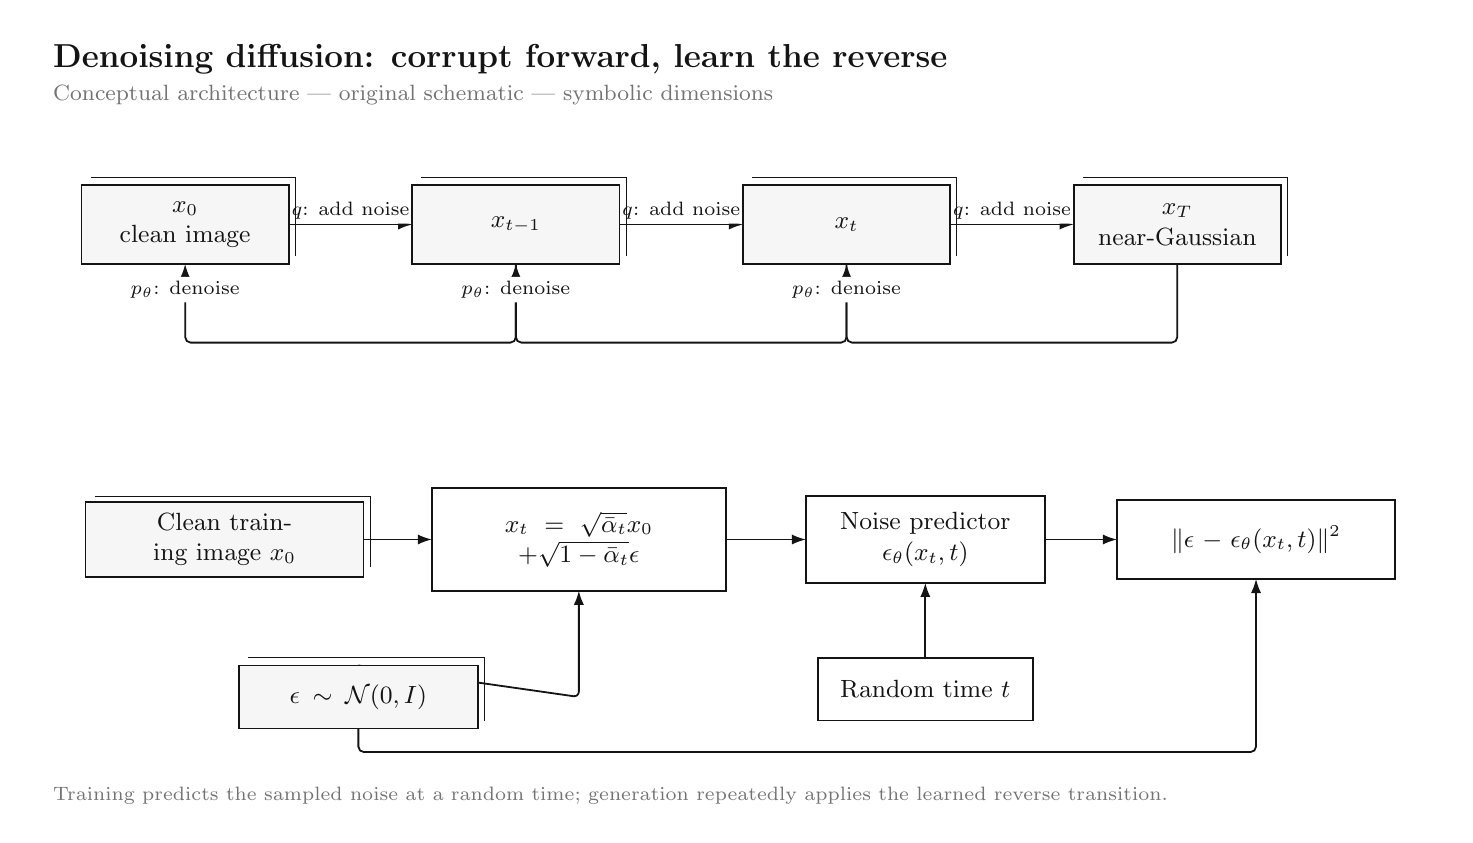
\begin{tikzpicture}[x=1cm,y=-1cm,font=\rmfamily,text=ink]

\path[use as bounding box] (0,0) rectangle (18,10);
\node[anchor=west,font=\large\bfseries] at (.2,.4) {Denoising diffusion: corrupt forward, learn the reverse};
\node[anchor=west,font=\footnotesize,text=soft] at (.2,.85) {Conceptual architecture | original schematic | symbolic dimensions};
\begin{pgfonlayer}{background}
\end{pgfonlayer}
\node[box,fill=wash,minimum width=2.6cm,minimum height=1.0cm,text width=2.35cm] (x0) at (2.0,2.5) {$x_0$\\clean image};
\draw[ink,line width=.4pt] (0.7999999999999999,1.9) -- (3.4,1.9) -- (3.4,2.9);
\node[box,fill=wash,minimum width=2.6cm,minimum height=1.0cm,text width=2.35cm] (xm) at (6.2,2.5) {$x_{t-1}$};
\draw[ink,line width=.4pt] (5.0,1.9) -- (7.6,1.9) -- (7.6,2.9);
\node[box,fill=wash,minimum width=2.6cm,minimum height=1.0cm,text width=2.35cm] (xt) at (10.4,2.5) {$x_t$};
\draw[ink,line width=.4pt] (9.2,1.9) -- (11.8,1.9) -- (11.8,2.9);
\node[box,fill=wash,minimum width=2.6cm,minimum height=1.0cm,text width=2.35cm] (xT) at (14.6,2.5) {$x_T$\\near-Gaussian};
\draw[ink,line width=.4pt] (13.399999999999999,1.9) -- (16.0,1.9) -- (16.0,2.9);
\node[box,fill=wash,minimum width=3.5cm,minimum height=0.9cm,text width=3.25cm] (clean) at (2.5,6.5) {Clean training image $x_0$};
\draw[ink,line width=.4pt] (0.85,5.95) -- (4.35,5.95) -- (4.35,6.8500000000000005);
\node[box,minimum width=3.7cm,minimum height=1.3cm,text width=3.45cm] (corrupt) at (7.0,6.5) {$x_t=\sqrt{\bar\alpha_t}x_0$\\$+\sqrt{1-\bar\alpha_t}\epsilon$};
\node[box,minimum width=3.0cm,minimum height=1.1cm,text width=2.75cm] (denoise) at (11.4,6.5) {Noise predictor\\$\epsilon_\theta(x_t,t)$};
\node[box,minimum width=3.5cm,minimum height=1.0cm,text width=3.25cm] (loss) at (15.6,6.5) {$\|\epsilon-\epsilon_\theta(x_t,t)\|^2$};
\node[box,fill=wash,minimum width=3.0cm,minimum height=0.8cm,text width=2.75cm] (eps) at (4.2,8.5) {$\epsilon\sim\mathcal N(0,I)$};
\draw[ink,line width=.4pt] (2.8000000000000003,8.0) -- (5.8,8.0) -- (5.8,8.8);
\node[box,minimum width=2.7cm,minimum height=0.8cm,text width=2.45cm] (time) at (11.4,8.4) {Random time $t$};
\begin{pgfonlayer}{background}
\draw[flow] (x0.east) -- (xm.west) node[midway,above,fill=white,inner sep=1.5pt,font=\scriptsize] {$q$: add noise};
\draw[flow] (xm.south) -- (6.2,4.0) -- (2.0,4.0) -- (x0.south) node[midway,above,fill=white,inner sep=1.5pt,font=\scriptsize] {$p_\theta$: denoise};
\draw[flow] (xm.east) -- (xt.west) node[midway,above,fill=white,inner sep=1.5pt,font=\scriptsize] {$q$: add noise};
\draw[flow] (xt.south) -- (10.4,4.0) -- (6.2,4.0) -- (xm.south) node[midway,above,fill=white,inner sep=1.5pt,font=\scriptsize] {$p_\theta$: denoise};
\draw[flow] (xt.east) -- (xT.west) node[midway,above,fill=white,inner sep=1.5pt,font=\scriptsize] {$q$: add noise};
\draw[flow] (xT.south) -- (14.6,4.0) -- (10.4,4.0) -- (xt.south) node[midway,above,fill=white,inner sep=1.5pt,font=\scriptsize] {$p_\theta$: denoise};
\draw[flow] (clean.east) -- (corrupt.west);
\draw[flow] (corrupt.east) -- (denoise.west);
\draw[flow] (denoise.east) -- (loss.west);
\draw[flow] (eps.north) -- (7,8.5) -- (corrupt.south);
\draw[flow] (eps.south) -- (4.2,9.2) -- (15.6,9.2) -- (loss.south);
\draw[flow] (time.north) -- (denoise.south);
\end{pgfonlayer}
\node[anchor=west,align=left,font=\scriptsize,text=soft,text width=17.6cm] at (.2,9.75) {Training predicts the sampled noise at a random time; generation repeatedly applies the learned reverse transition.};
\end{tikzpicture}
\end{document}
